\chapter{LHC and CMS experiment}

The Large Hadron Collider~\cite{LHC_refer} is the most powerful hadron collider ever built. The circumference of this circle superconducting collider is 26.7 km and the designed full operation energy is 14 TeV. In 2012, the LHC operated on 8 TeV and in 2016, it boosted up to 13 TeV. There are four collision locations on the LHC ring which hold four particle detectors, ALICE, ATLAS, CMS and LHCb. The ATLAS and CMS are general purpose detectors, aiming for the high luminosity operation . The LHCb focuses on the b physics study, while ALICE studies the lead-lead collision.
%in the order $L=10^{34} cm^{-2}s^{-1}$%
\section{LHC accelerator}

A sketch view of the proton accelerating process is shown in Figure.~\ref{fig:LHC_sketch}. The LHC is the most powerful accelerator in the accelerating chain. Before the beams are injected into the LHC, a series of steps are taken. In the proton-proton(p-p) collision, protons are from the source Duoplasmatron, which uses electric field to break down hydrogen gas into protons and electrons, then the protons are accelerated by a 90 kV supply. Leaving the source, the protons are focused and accelerated to 750 keV by the radio frequency quadrupole. Then the protons are further accelerated by linear accelerator Linac2 to 50 MeV. The proton synchrotron booster further accelerates the protons from 50 MeV to 1.4 GeV and injects the protons into the proton synchrotron(PS). The PS accelerates the protons to 25 GeV followed by the super proton synchrotron which boosts the protons to 450 GeV. The LHC is the last ring in the whole accelerating process and accelerates the protons to its current final energy 6.5 GeV. In a normal fill of protons in LHC, the ring holds 2808 bunches with an approximation of $10^{11}$ protons.

There are thousands of superconducting magnets along the LHC ring to bend and focus the beam. Among the magnets, there are 1232 main dipoles which are used to bend the beam with a magnetic field above 8 T. Other types of magnets, for example, the quadrupole magnet can tight the beam either vertically or horizontally, while the sextupole, octupole and decapole can help fine tuning the magnetic field. The radiofrequency cavities(RF) in the LHC are used to accelerate the protons from 450 GeV to 6.5 GeV, keep the bunches in the beam pipe compact and restore the energy loss from synchrotron radiation. Eight RFs per beam, provide 16 MV  longitudinal oscillating voltage with the 400 MHz superconducting cavity system. 

The machine luminosity is an important parameter of the collider. For a process under study, the number of events created per-second $N_{\textrm{event}}$ is shown in Equation.~\ref{event_number}, in which L is the machine luminosity and $\sigma_{event}$ is the cross section of that process.

\begin{align}\label{event_number}
N_{\textrm{event}}=L\sigma_{event}
\end{align}

The machine luminosity is determined by a number of factors as shown in Equation.~\ref{Lumi_express}. The $n_b$ and $N_{b}$ are the number of bunches per-beam and the number of protons per-bunch respectively. The $f_{rev}$ and $\gamma_{\gamma}$ are the revolution frequency and relativistic gamma factor respectively. The $\beta*$ is the amplitude function of the beam at the collision point while the function F describes the reduction of luminosity because of the crossing angle. This machine luminosity is also called instantaneous luminosity which is the luminosity at a unite time. The integrated luminosity which later is referred as luminosity is the instantaneous luminosity that integrates over time~\ref{fig:LHC_sketch}.  

\begin{align}\label{Lumi_express}
L=\frac{N_{b}^{2}n_{b}f_{fev}\gamma_{\gamma}}{4\pi\epsilon\beta*}F
\end{align}



\begin{figure}[htbp] 
\centering
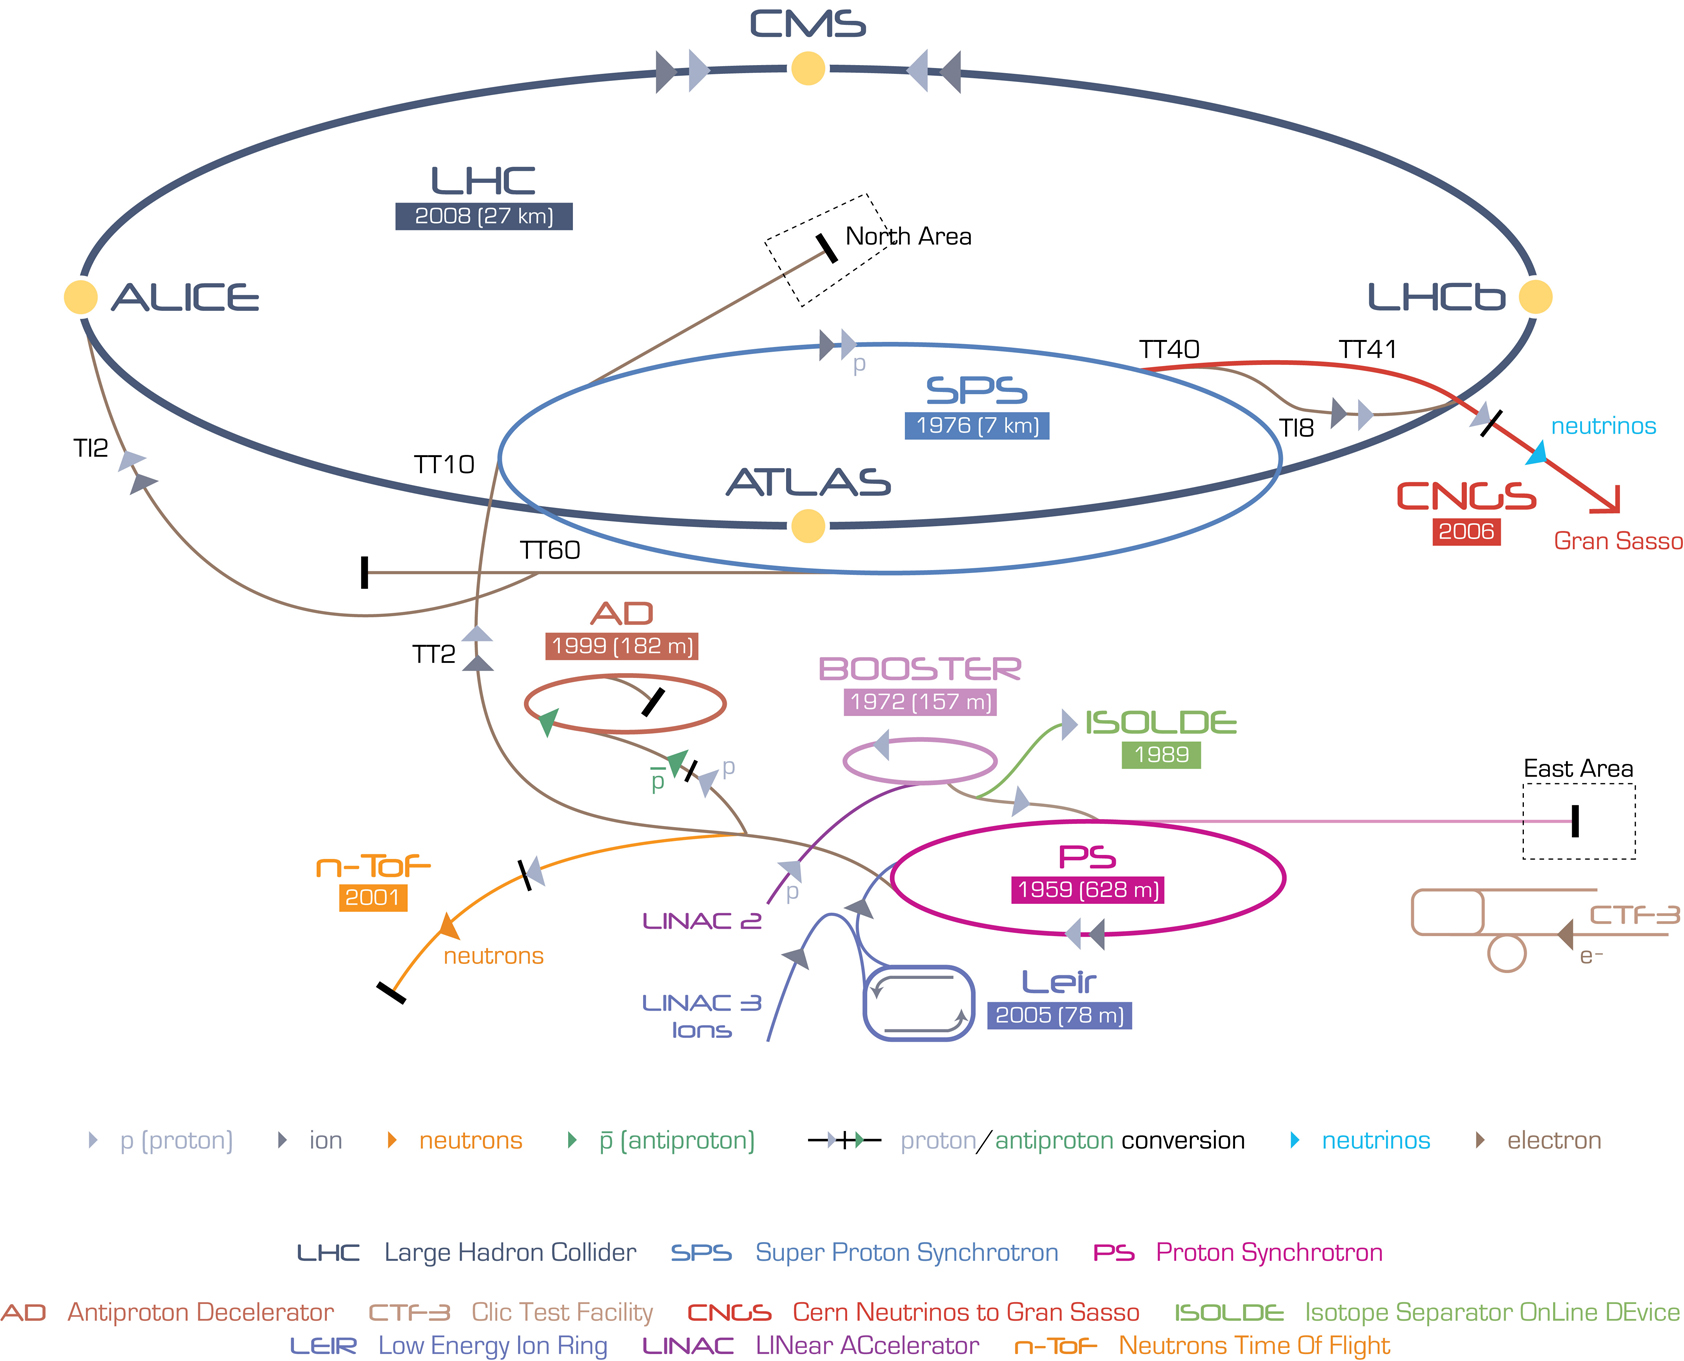
\includegraphics[width=0.8\textwidth]{chapter3/LHC_chain.jpg}
\caption{A sketch view LHC injection chain and main experiments associated~\cite{Christiane:1260465}.}
\label{fig:LHC_sketch}
\end{figure}


\section{Compact Muon Solenoid}
The compact muon solenoid(CMS) is a general purpose detector. It is a high performance detector that is designed to observe any new physics produced by LHC. It covers a broad range of physic studies like the standard model physics and the search for supersymmetry and dark matter candidates. The CMS detector is designed to have good muon momentum and position resolution over a large range of energy and angles, good charged particle momentum resolution and high identification efficiency within inner tracker, good electromagnetic energy and position resolution, high photon and lepton isolation efficiency in high luminosity condition and good missing transverse momentum and jet energy resolution.  


An general view of the CMS detector is shown in Figure.~\ref{fig:CMS_sketch}. The detector is composed of a set of sub-detectors from the inside and out in a ring structure. The main sub-detectors are the followings:

\begin{figure}[htbp] 
\centering
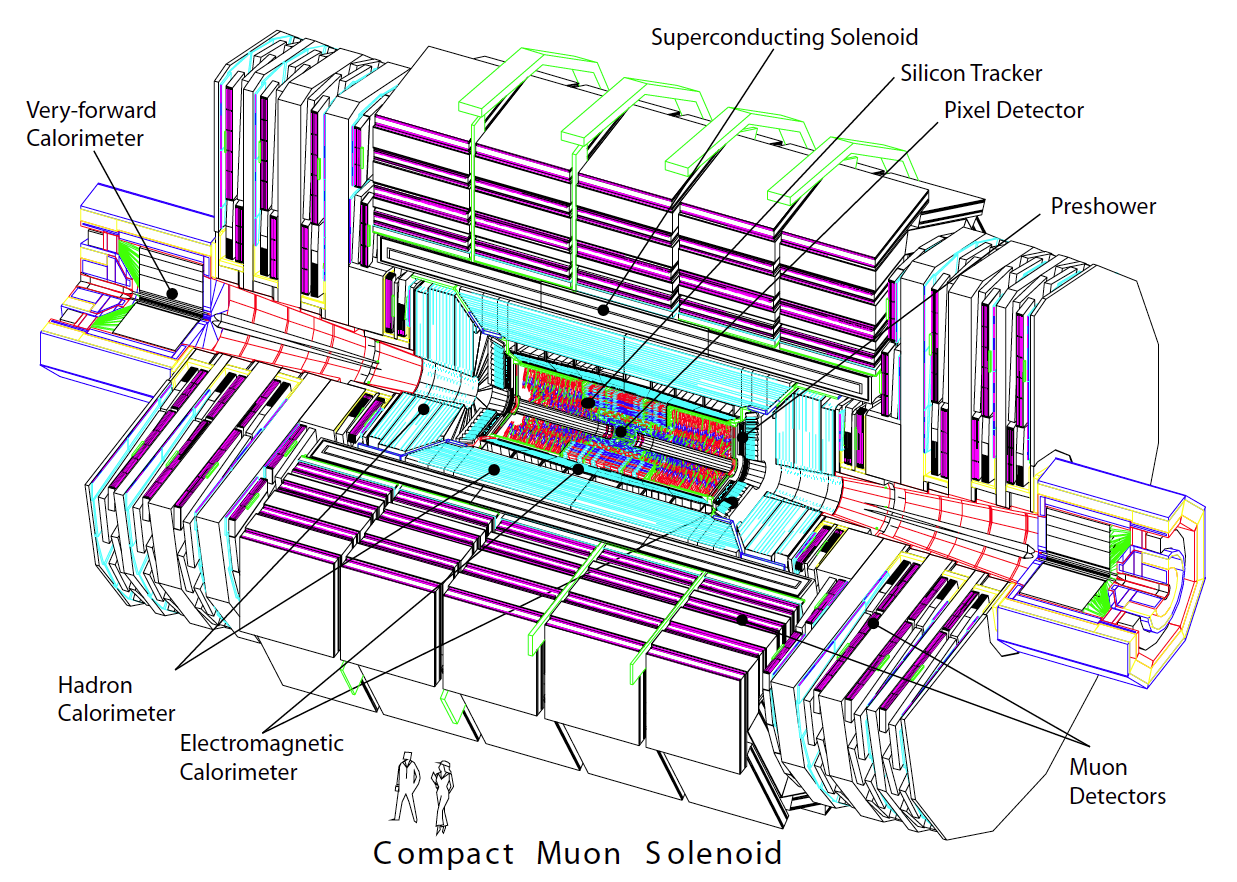
\includegraphics[width=0.8\textwidth]{chapter3/CMS_detecter.png}
\caption{A sketch view of CMS detector~\cite{CMS_experiment}}
\label{fig:CMS_sketch}
\end{figure}


\begin{enumerate}[$\bullet$]
\item The inner tracker consists of two parts, the pixel detector and silicon strip tracker which are used measure the momentum and tracks of the charged particles.
\item The electromagnetic calorimeter mainly measures the energy and the position of electrons and photons. Other particles will leave some percentage of energy inside while passing through.
\item The hadron calorimeter measures the energy of hadrons. 
\item The muon detector measures the tracks and momentum of the muons.
\end{enumerate} 

Another outstanding feature of CMS is the superconducting magnet system, which provides a 3.8 T magnetic field. The configuration of the magnet system drives the design and layout of the detector. Besides the sub-detectors listed above, trigger system is also crucial for the success of the whole program. The trigger system consists of two parts, the hardware based level one trigger and the software based high level trigger. The trigger system does the initial selection of interesting events from a huge flux of events per-collision, which makes it possible for data-acquisition and recording. The details of the sub-detectors and other systems mentioned will be further discussed later. 

In general, the CMS detector is 21.6 m long, 14.6 m in diameter and weighs 12500 tonnes in total. The coordinate system adopted by CMS sets the center at the collision point. The x-axis points towards the center of LHC ring and the z-axis points along the beam direction. The azimuthal angle $\phi$  measures from the x-axis in the x-y plane, polar angle $\theta$ measures from the zenith direction  and the r is the radial coordinate. Another variable called the pseudorapidity $\eta$, defined as $\eta=-\textrm{ln}\big[\textrm{tan}(\theta/2)\big]$ is also frequently used in the measurement. In the case, a particle with $E\gg m$, pseudorapidity can be approximated as $\eta=-\textrm{ln}\big(\frac{E+p_{z}}{E-p_{z}}\big)$, where the $p_{z}$ is the longitudinal component of momentum~\cite{CMS_experiment}. 

\subsection{Tracker}
The inner tracking system of CMS is designed to measure the trajectories of charged particles. The efficient and precise measurement is crucial for the reconstruction and identification of particles. The LHC operates with the instantaneous luminosity in the order of $10^{34}cm^{-2}s^{-1}$, in average producing more than 20 p-p interactions and 1000 particles per-bunch crossing collison. High granularity and fast response are the primary features of the tracker system. To measure the trajectories precisely, low interactions of tracker materials with incoming particles, like multi-scattering, photon conversion and nuclear interaction are also important. In the long operation period, radiation hardness of the tracker material is needed. All of these factors drive the design of CMS tracker system.

The tracker system of CMS surrounds the collision point and has the dimension of 5.8 m in length and 2.5 m in diameter, with a coverage up to pseudorapidity $|\eta|<2.5$. A overview of the tracker system layout is shown in Figure.~\ref{fig:tracker_sketch}. Three layers of silicon pixel detector modules surround the interaction point and two additional disks of pixel modules on each side, in all 66 million pixels of the size $100\times150~ \mu m$ each. Following the pixel detector is the silicon strip tracker. There are four components of the strip tracker, tracker inner barrel(TIB), tracker inner Discs(TID), tracker outer barrel(TOB) and tracker end caps(TEC). The arrangement of the strip tracker components is shown in Figure.~\ref{fig:tracker_sketch} which consist of 10 layers and about 10 million strips. 


\begin{figure}[htbp] 
\centering
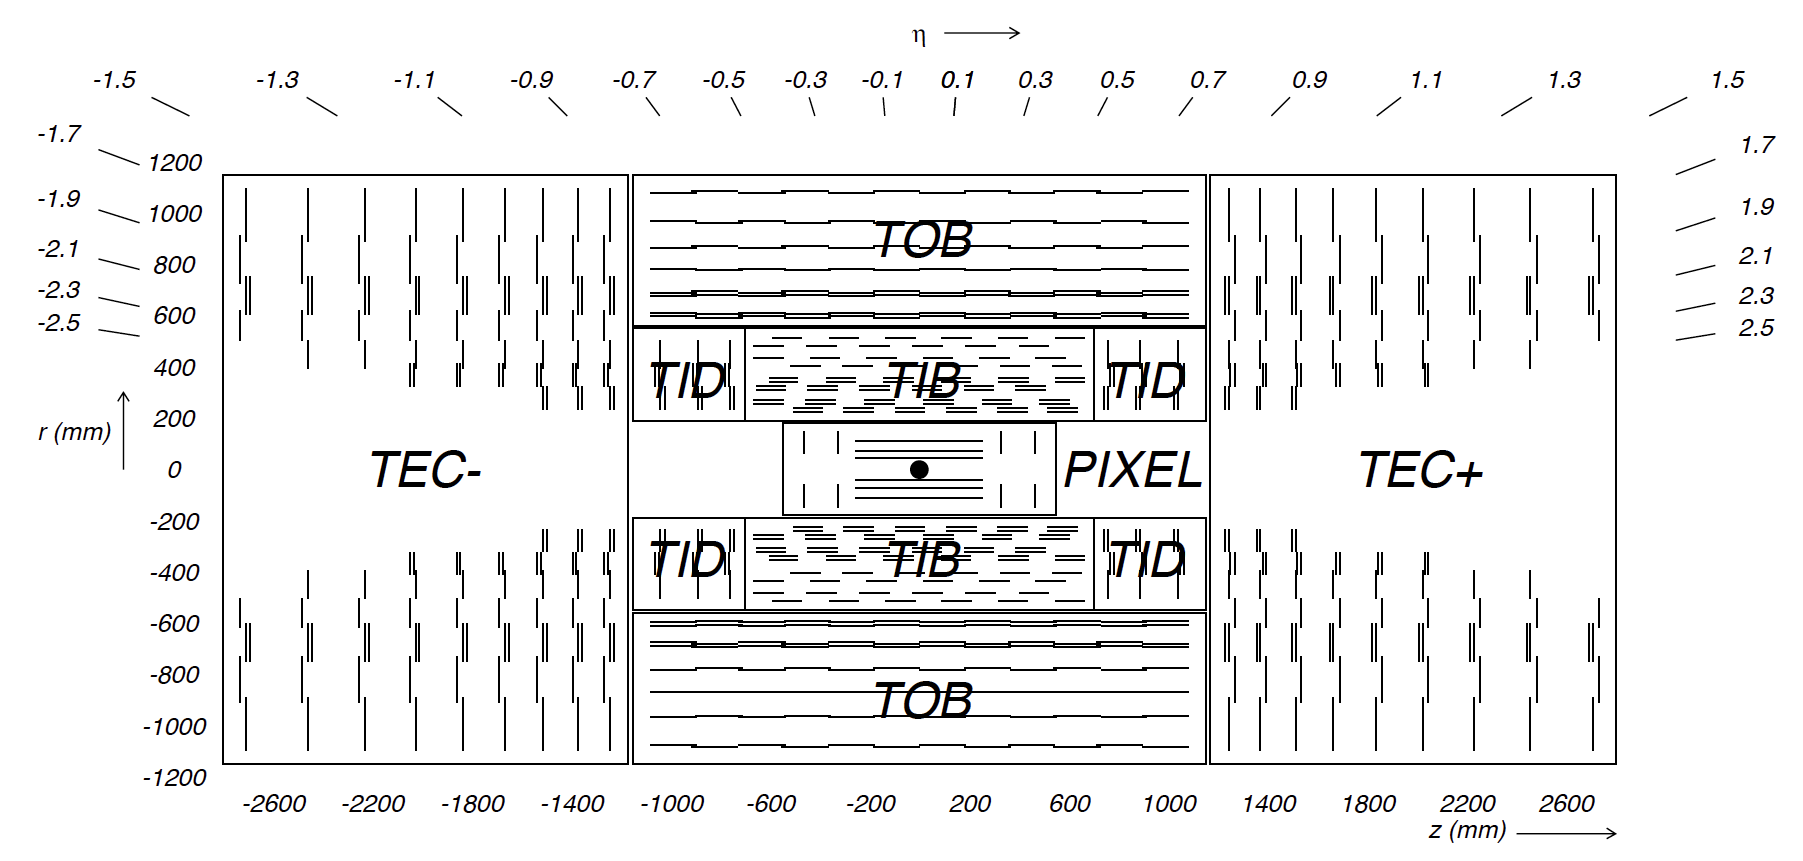
\includegraphics[width=0.8\textwidth]{chapter3/Tracker_structure.png}
\caption{The structure of tracker in CMS~\cite{CMS_experiment}}
\label{fig:tracker_sketch}
\end{figure}



\subsection{Electromagnetic calorimeter}

The electromagnetic calorimeter(ECAL) in CMS is a hermetic homogeneous lead tungstate($\textrm{PbWO}_{4}$) detector. The whole sub-detector is composed of two parts, the central barrel(EB) covering the pseudorapidity range $|\eta|<1.479$ and the endcap disks(EE) covering the range $1.479<|\eta|<3.0$. The EB is made up of 61200 $\textrm{PbWO}_{4}$ crystals with $22\times22~mm^{2}$ in the front face, 23 cm in length(25.8 in radiation lengths). The EE is made up of 7324 crystals per disk with front face $29\times29~mm^{2}$, 22 in length(24.7 in radiation lengths) and a preshower detector(ES)~\cite{CMS_TDR}. The geometrical configuration of ECAL is shown in Figure.~\ref{fig:ECAL_sketch}. 

The $\textrm{PbWO}_{4}$ crystals used in ECAL have high density(8.28 $g/cm^{3}$), short radiation length(0.89 cm) and small Moli$\grave{e}$re radius(2.2 cm), together with the specific geometrical parameters used, rendering ECAL  good energy resolution, fast response, fine granularity and high radiation resistant. Photodetectors are placed at the end of the crystals. In EB, avalanche photodiodes(APDs) are used, while vacuum phototriodes(VPTs) are used in EE. Both types of the photodiode show good performance in the environment with hard radiation and 4 T magnetic field. The ES is in front of the EE in the pseudorapidity range $1.653<|\eta|<2.6$. The ES is a sampling detector with silicon strip sensors placed behind the lead radiator to measure the energy and position of the incoming particles.  

\begin{figure}[htbp] 
\centering
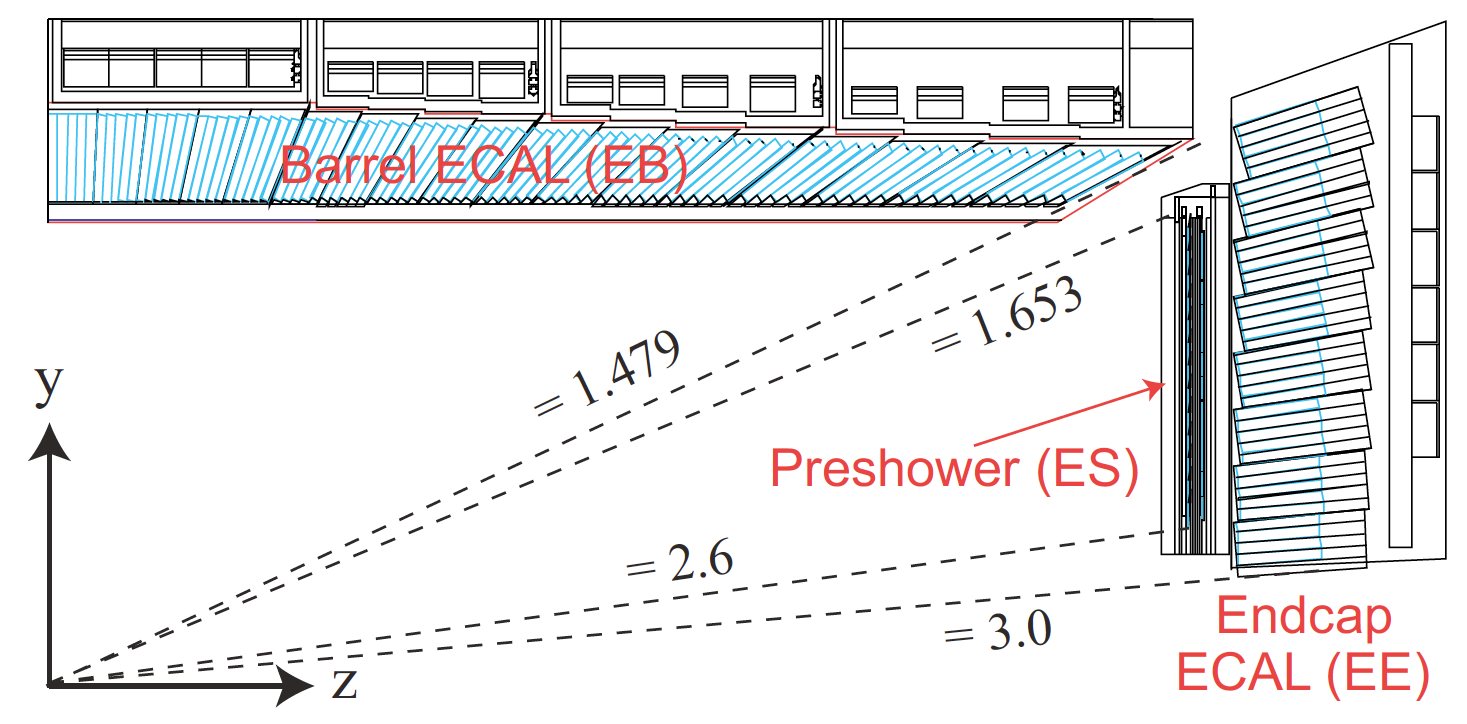
\includegraphics[width=0.8\textwidth]{chapter3/ECAL_transverse.png}
\caption{ECAL geometrical configuration~\cite{CMS_TDR}}
\label{fig:ECAL_sketch}
\end{figure}

Each half of the EB is composed of 18 supermodules that each supermodule contains 1700 crystals. The relative energy resolution of $\textrm{PbWO}_{4}$ crystal  refers to the resolution that is measured with ECAL supermdules directly exposed to electron beam without considering the materials in front. The relative energy resolution as a function of electron energy can be expressed as 
%spikes
% np scattering in the protective epoxy coating of the APD, and the resulting proton directly ionizing the APD active volume.
\begin{align*}
\frac{\sigma}{E}=\frac{2.8\%}{\sqrt{E/\textrm{GeV}}}\oplus\frac{12\%}{E/\textrm{GeV}}\oplus 0.3\%
\end{align*}

The first term stands for the contribution from stochastic factors, like the number fluctuation in production of the secondary particles. The second term is the noise contribution coming from the electronics and digitization, while the last is a constant term that covers the other contribution factors~\cite{ECAL_EB_reso}.

\subsection{The hadron calorimeter}

The CMS hadron calorimeter(HCAL) is a hermetic sampling detector, which is important for the measurement of the energy and momentum of hadrons, also the missing energy that caused by the non-interacting particles.  The HCAL is composed of three parts, the HCAL barrel(HB), HCAL endcaps(HE) and forward calorimeter(HF). The mechanical structure of HCAL is shown in Figure.~\ref{fig:HCALL_sketch}. 

\begin{figure}[htbp] 
\centering
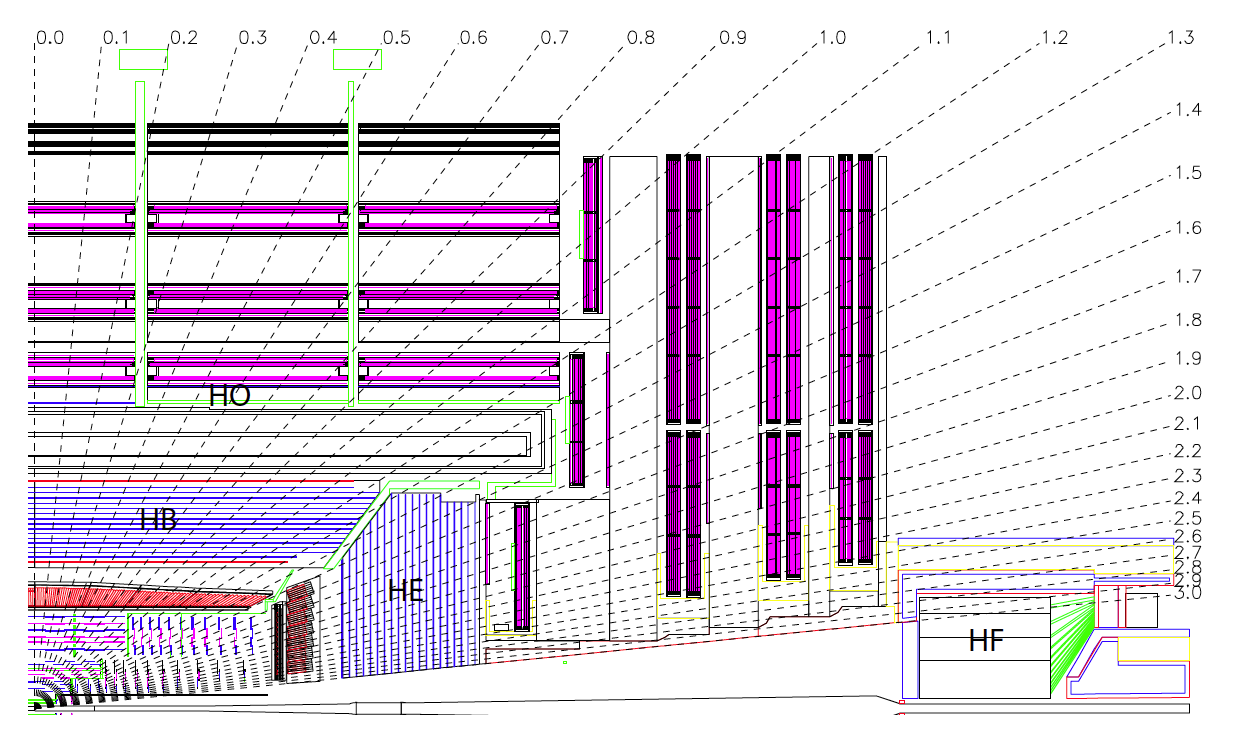
\includegraphics[width=0.8\textwidth]{chapter3/HCAL_sketch.png}
\caption{A longitudinal view of CMS HCAL sub-detector~\cite{CMS_experiment}}
\label{fig:HCALL_sketch}
\end{figure}


The HB is composed of  several layer of brass absorber plates, between which are the plastic scintillator tiles. The innermost and outermost layer plates are made of stainless steel to gain structural strength. When hadrons hit the absorber, secondary particles are produced in showers. As the showers develop, the alternating layers of scintillators are activated and emit blue-violet light. The lights are collected as signals. The HB covers the central pseudorapidity range $|\eta|<1.3$ with an individual read out unit $\Delta \eta\times\Delta\phi=0.087\times 0.087$. Because of the limited spaces between ECAL and muon detector, to have enough sampling depth in HCAL central region, an extra outer calorimeter(HO) is installed. The HO utilizes the outside solenoid coil as additional absorber to insert plastic scintillators. Similar to the HB, the HE is also made of brass absorber and plastic scintillator tiles layers, which covers the range $1.3<|\eta|<3.0$. The read out units have the geometry $\Delta \eta\times\Delta\phi=0.17\times 0.17$ in HE~\cite{CMS_experiment}. A combined ECAL and HCAL energy resolution~\cite{HCAL_reso} measured in test beam with pions is 

\begin{align*}
\frac{\sigma}{E}=\frac{110\%}{\sqrt{E/\textrm{GeV}}}\oplus 0.9\%
\end{align*}

The HF situates $\pm11$ m from the interaction point to complement the large pseudorapidity measurement of HE in the range $3.0<|\eta|<5.0$. The HF is made of grooved steel plates with quartz fibers. Charged shower particles generate Cherenkov light, which is collected by the quartz fibers as signals. Radiation hardness is critical for the operation of HF.   



\subsection{Muon detector}
The CMS muon detector is designed to measure the momentum and charge of muon. Three types of gas detectors are used in CMS, the barrel drift tube(DT) chambers, the cathode strip chambers(CSC) in the endcaps and the resistive plate chambers(RPC) in both barrel and endcap regions. 

In the muon detector barrel(MB), DT chambers and RPCs are used which covers the pseudorapidity region $|\eta|<1.2$. The MB is composed of 250 chambers. The chambers are located in 4 stations inside the magnet return yoke. The yoke is further divided into 5 wheels, each of which is composed of 12 sectors. As shown in Figure.~\ref{fig:muon_sketch}, the stations are named MB1 to MB4, which are composted of one DT chamber and varied number of RPCs that depending on the exact location. DT chambers measure the position of the incoming muons which knock off the electrons in the gas atoms of the chambers and are collected by a large numbers of charged wires inside.% The gas used in DT chambers is a mixture of Ar and $\textrm{CO}_{2}$.

In muon detector endcaps(ME), 468 CSCs which covers the range $0.9<|\eta|<2.4$ are used. The MEs are also composed of 4 stations of chambers in each of the discs. The CSCs are in a wedge shape and composed of 6 gas gaps. Each gap is filled in with a cathodes strip and anode wires which run perpendicularly to the strip. Incoming muons knock off the electrons and create avalanches which are received by the positive charged wires. 

Both DT chambers and CSCs measure the position and trigger on the $\pt$ of muons. To better deal with the high luminosity and improve the $\pt$ resolution of the triggered muon, a dedicated trigger system, the RPCs are added to both MB and ME. RPCs are double-gap bakelite chambers which operate with the avalanches that caused by the muons. RPCs can provide additional fast triggering and sharp $\pt$ triggering thresholds. Four RPCs layers are used in the MB first two stations(two each) and another two layers(one each) are used in the last two stations.  In the ME, one RPC layer in each of the first three stations.    



\begin{figure}[htbp] 
\centering
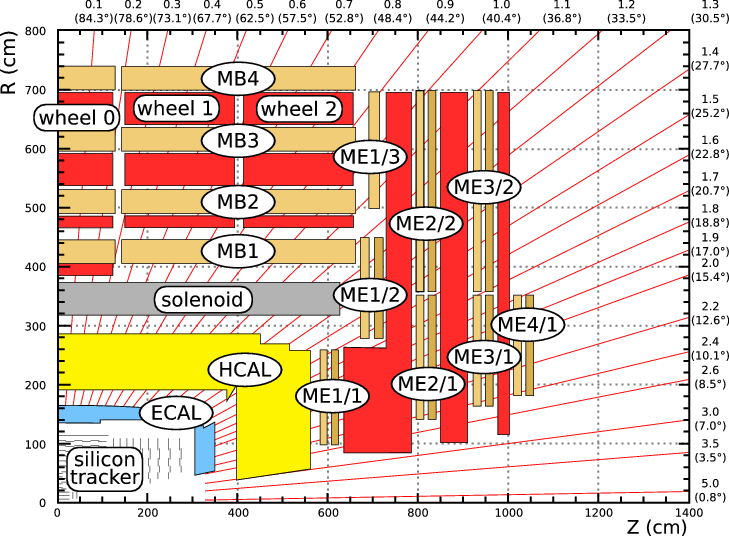
\includegraphics[width=0.8\textwidth]{chapter3/Muon_chambers.png}
\caption{A overview of muon chamber configuration in CMS~\cite{Muon_chambers}}
\label{fig:muon_sketch}
\end{figure}


\subsection{Trigger}

The LHC is a high luminosity collider in the order of $10^{34}\textrm{cm}^{2}\textrm{s}^{-1}$. In the p-p collision, the bunch crossing time is 25 ns and the corresponding frequency is 40 MHz. In each of the 25 ns, there are approximately 20 collisions. This high rate makes it impossible to transmit and record all of the events, also it is not necessary, since most of the events are not of current physics research interests. The CMS use a two level trigger system to select events and reduce the event recording rate, the Level-1(L1) trigger and High-level trigger(HLT) systems. 


The L1 trigger system is based on custom designed and programmable electronics which are situated inside the detector. It utilizes the information from calorimeters and muon system, performing simplified but effective reconstructions, corrections and selections. The L1 reduces the event rate from 40 MHz to 100 kHz. In LHC Run II, the L1 trigger system has been upgraded to deal with the increasing luminosity and improves the performance. The L1 calorimeter trigger accesses the information from the whole ECAL and HCAL in the granularity of trigger tower level, which approximately corresponds to a region $0.087\times0.087$ in $\eta$ and $\phi$. The L1 trigger reconstructs the $\Pe/\gamma$, jets, $\tau$ and the sum energy of the candidates with the algorithms implemented in the time multiplexed trigger architecture~\cite{TMT_trigger}. The algorithms are implemented at hardware trigger level, with dynamic clustering of trigger towers, pile-up migration and innovated tau and jet reconstruction with various look-up table for the calibrations and corrections~\cite{L1_Egamma}. The L1 muon trigger system fully utilizes three muon detectors in the track reconstruction. In general, the track reconstruction of muons are divided into three regions, the barrel, the overlap and the endcap, based on the geometry. Through dedicated construction algorithm, tracks are built, so as computing the muon qualities. These informations are used in the triggering processes~\cite{L1muontrigger}. 


The HLT in CMS further reduces the event rate from 100 kHz(after L1 trigger selection) down to 1 kHz. The HLT is software based trigger system and utilized the streamlined version of the CMS soft-ware for event reconstruction on the large computer farm~\cite{CMS_trigger_RUNII}. Maximizing the trigger efficiency and keeping acceptable CPU-time is crucial for the HLT system. The HLC accesses to the full granularity and sub-detectors of CMS, including the tracker. The dedicated algorithms used in the HLT is the very closed to the ones used in the off-line reconstruction and analysis, besides some of the parameter configurations~\cite{CMS_HLT_RunII}.             








%\subsubsection{Level 1 Trigger}
%probably I have to put something there2



%\subsubsection{High Level Trigger}

